\section{Analysis}
\label{sec:analysis}

This section details the analyses performed on the data. The analyses mimic the ROUGE-1,2 and L methods of comparing documents, where we compare the tweet and article text using these methods. This is done to determine whether the tweets promoting the articles could be generated from the document text. The results of the comparison show that the tweet is not extracted from the article text. 

We calculate the degree of common words - unigrams and bigrams, between the tweet and the text of the document. We also check least common subsequences between the tweet and the document. These are the ROUGE-1,2 and L style calculations. The hypothesis is that these results give an approximation of the degree to which the tweet is extracted from the document text. 

For all these analyses, the stop words have been eliminated from the tweet as well as the document, so that only the significant words are taken into consideration. The hashtags, references (@) and URLs from the tweets were also all removed.

\subsection {Tweet extracted directly from article}
To calculate the position of tweet text as a whole in the text, we checked for a complete substring match of the tweet in the text. Out of the 2471 unique instances of tweet and article pairs, a complete match was found 23 times. 9 times out of these, the tweet text had been matched against title of the article extracted into the text. The rest of the results are significant, since the text of the tweet appears exactly as is inside the text of the article. This suggests that the user chose the sentence that either seemed to be the most conclusive contribution of the article, or expressed the opinion of the user to be tweeted.

Apart from the 9 times that the tweet was matched with text in the article, we also checked to see if the tweet text matched with the article titles that were separately extracted with the newspaper package. We found that it didn't match with the titles. This comparison shows that the tweet is extracted from the article very few times, and does not match with the title of the articles a lot of times either. 

\subsection{Percentage match for unigrams}

Next, we did a percentage match with the text of the article. This was a bag-of-words check using unigrams from the tweet and the document. The order of the words in the tweet or the text did not matter. The results we got seem to suggest that a lot of significant words in the tweet are in fact present in the article. The minimum percentage match obtained was 60\%. However, since the order of the words did not matter, this result can  be traced back to the fact that tweet is based on the same topic as the document. \figref{fig:unigrammatch} shows the percentage of matches in the tweet and the article text as compared to the number of unigrams in the tweet. The mean of the match percentages is 29.53 and standard deviation is 20.2. The graph shows that if compared to the unigrams in a tweet, the number of unigrams matched from that tweet is not consistently high for the tweet describing the article. \figref{fig:num_unigrams} shows the number of articles with same number of matching unigrams. The graph shows maximum number of articles with 2 unigrams matched. The number of articles with more unigrams matched goes on decreasing. The slight rise at the end - more than 10 matched unigrams - is accounted for by the completely matched tweets described above. Let $\textit{unigrams}(x)$ be the set of unigrams for some text $x$, then $u$, the percentage of matching unigrams found between a given tweet, $t$ and a given article, $a$, can be defined as  

\begin{equation}
u = \frac{| unigrams(t) \cap unigrams(a) |}{| unigrams(t) |} * 100
\end{equation}

\begin{figure}[htbp]
\centering
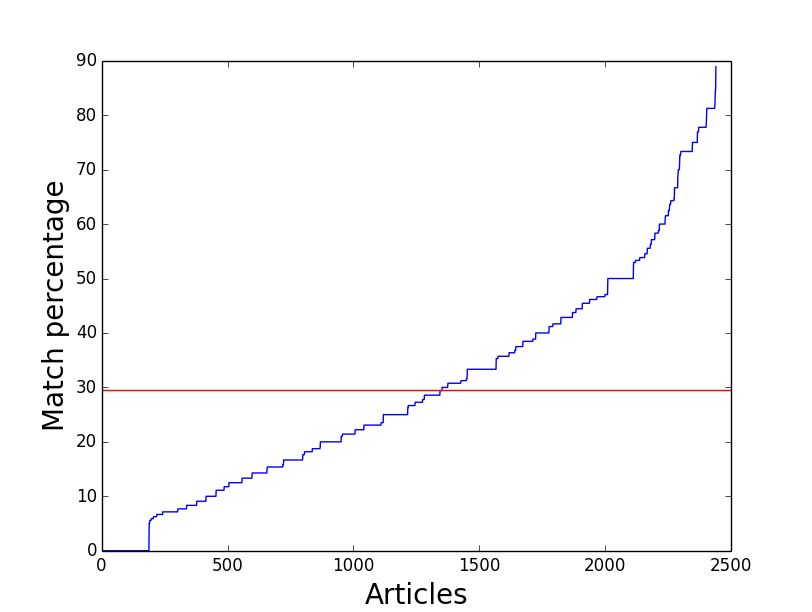
\includegraphics[width=0.5\textwidth, height=6cm]{unigrammatch}
\caption{Distribution of unigram match percentage over unique tweets and articles.}
\label{fig:unigrammatch}
\end{figure}

\begin{figure}[htbp]
\centering
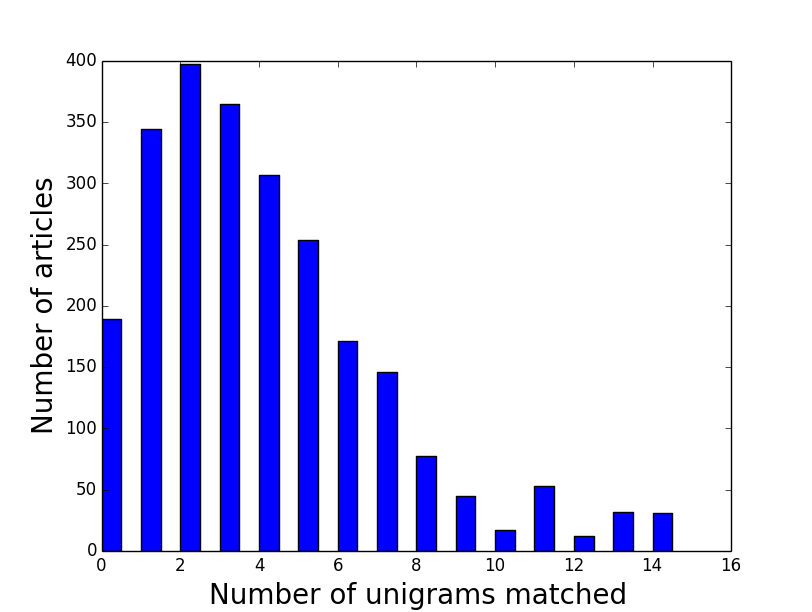
\includegraphics[width=0.5\textwidth, height=6cm]{num_unigrams}
\caption{Histogram of number of unique tweet-article pairs vs number of unigrams matched. The mean number of unigrams matched per tweet-article pair is 3.9.}
\label{fig:num_unigrams}
\end{figure}

\subsection{Percentage match for bigrams}

Similar to the unigram matching techniques, bigram percentage matching was also calculated. The text of the tweet was converted into bigrams and we then looked for those bigrams in the article text. The percentage was calculated similar to the unigram matching done earlier. \figref{fig:num_bigrams} shows frequency of the number of tweet-article pairs for the number of bigrams matched. There are no matched bigrams for most of the pairs. The number then decreases from one matched bigram till the end, where it increases a little at more than 10 matched bigrams, similar to the unigram frequency graph. For the set of bigrams for a text $x$, $\textit{bigrams}(x)$, percentage of matching bigrams $b$ for the tweet $t$ and article $a$ is calculated as 

\begin{equation}
b = \frac{| bigrams(t) \cap bigrams(a) |}{| bigrams(t) |} * 100
\end{equation}

\figref{fig:bigrammatch} shows the percentages of matched bigrams found in every article. Mean is 10.73 with a standard deviation of 18.5. As seen in the figure, most of the tweet-article pairs have no matched bigrams. The percentage then increases to reflect the complete matches found above.

\begin{figure}[htbp]
\centering
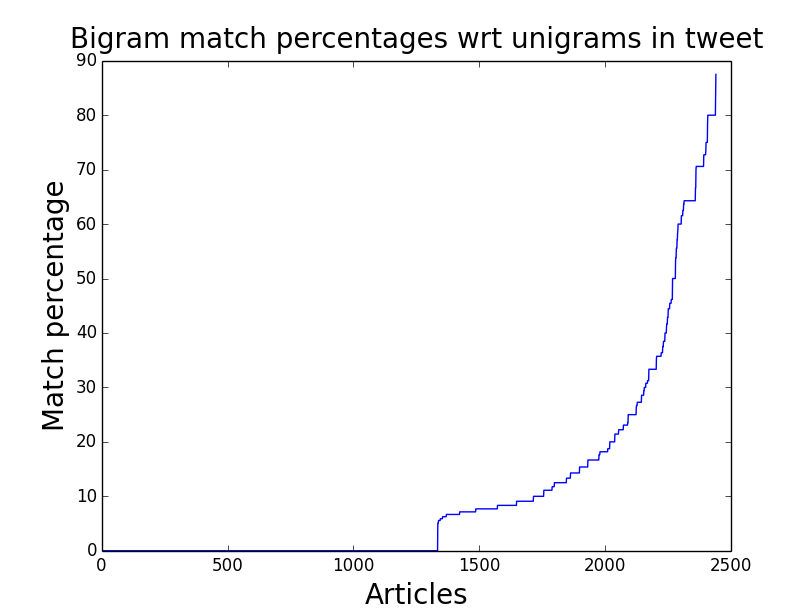
\includegraphics[width=0.5\textwidth, height=6cm]{bigrammatch}
\caption{Distribution of bigram match percentage over the tweet-article pair.}
\label{fig:bigrammatch}
\end{figure}

\begin{figure}[htbp]
\centering
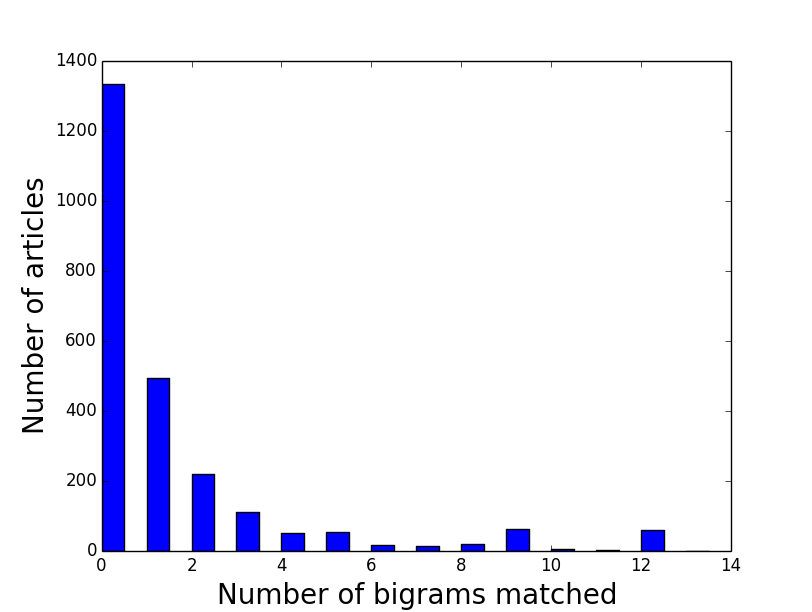
\includegraphics[width=0.5\textwidth, height=6cm]{num_bigrams}
\caption{Histogram of number of unique tweet-article pairs vs number of bigrams matched. The mean number of bigrams matched per article is 1.9.}
\label{fig:num_bigrams}
\end{figure}

\subsection{Percentage matching inside a window in the article text}

The next analysis was to check for a significant word matching inside a three sentence window inside the article text. We used a three sentence long window using the sentence boundary information obtained during preprocessing. A window of three sentences was chosen to give a smaller context for the tweet to be extracted from than the entire article. The number was chosen as a moderate context window size as not too small to reduce it to a sentence level, and not too big for the context to be diluted. 

After the text of the window was extracted, we performed a similar analysis as the last one, except on a smaller set of sentences. Again, the order of the unigrams didn't matter. Next, the matching percentages from all such windows in the articles were compared and the maximum out of these was considered for the highest match percentage and match position for the final results. The result from this experiment is shown in \figref{fig:unigramwindow}. Here, the mean of the values is 26.6\% and deviation 17\%. Let a sentence window $w_i$ be the set of three consecutive sentences starting from the sentence number $i$. For this window, the unigram match in the tweet $t$, and the window is the unigram match $u$ calculated above. Then, the maximum match from all the windows, $uw$ is 

\begin{equation}
uw = max \left( \bigcup_{w_i \in S} u \left( t, w_i \right) \right)
\end{equation}

\begin{figure}[htbp]
\centering
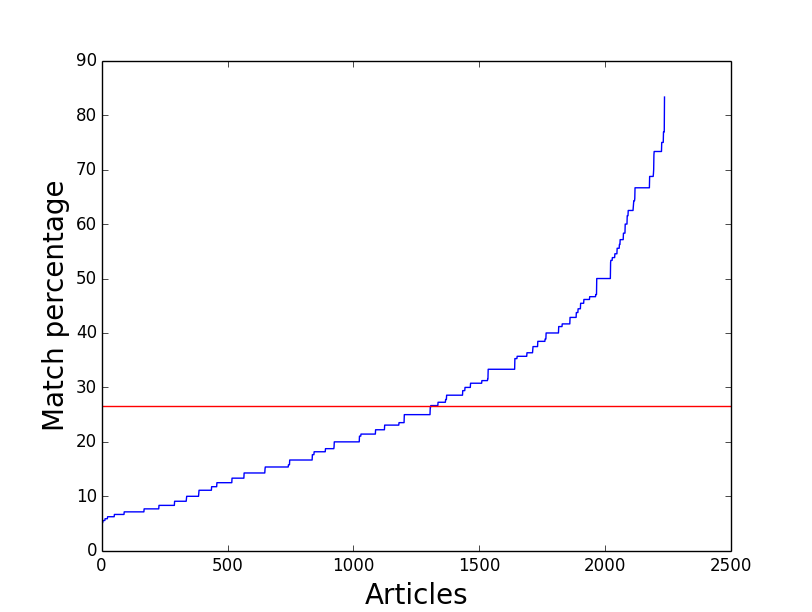
\includegraphics[width=0.5\textwidth, height=6cm]{unigramwindow}
\caption{Percentages of common words in tweet and a three sentence window in the aritcle. The maximum match from all percentages is chosen for an article.}
\label{fig:unigramwindow}
\end{figure}

\subsection{Longest Common Subsequence match inside a window for the text}

The percentage match analyses were a bag-of-words approach disregarding the order of the words inside the texts and tweets. To respect the order of the words in the sentence of the tweet, we also used the least common subsequence algorithm between the tweet text and the document text. This subsequence matching was done inside a sentence window of 5 sentences. Again, the final result for the article was the window in which the maximum percentage was recorded among all windows. The percentage match was calculated against the number of words in the tweet, as found in the least common subsequence calculated between the two texts. These numbers are shown in \figref{fig:lcs}. The mean here is 44.6\% and the standard deviation is 22.7\%. If $\textit{lcs(t, a)}$ is the longest common subsequence between the tweet $t$ and article $a$, $\textit{unigrams}(x)$ is the set of unigrams for a text $x$, then the percentage of match for the lcs as compared to the tweet, $\textit{l}$ is

\begin{equation}
l = \frac{| lcs(t, a) |}{| unigrams(t) |} * 100
\end{equation}

\begin{figure}[htbp]
\centering
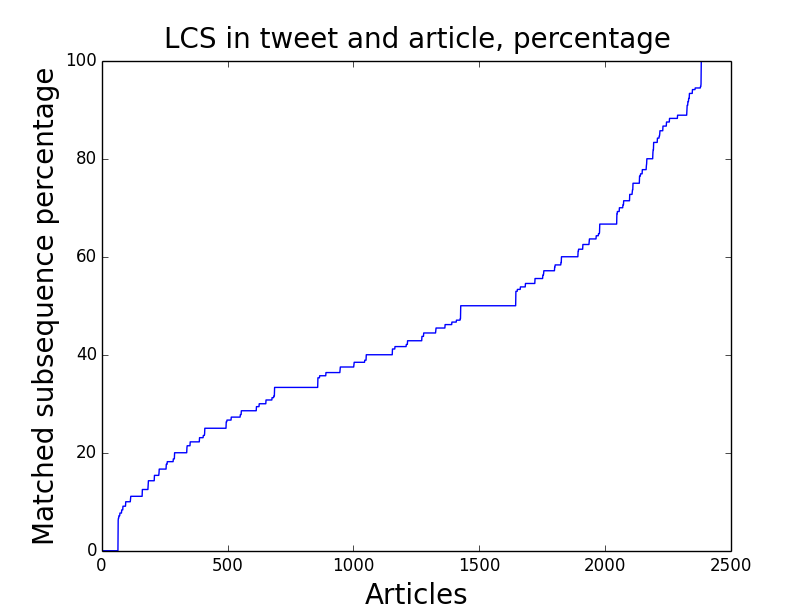
\includegraphics[width=0.5\textwidth, height=6cm]{lcs_doc}
\caption{Percentages of words matching in tweet and document text using an LCS algorithm.}
\label{fig:lcs}
\end{figure}